\chapter{Omisión de palabras}

Anteriormente se especificó que la base de datos de los préstamos serían únicamente palabras de contenido, y a partir de ellas se realizaron los análisis anteriores.  Al trabajar con esta clasificación se están restringiendo a todas las palabras que pueden ser catalogadas como préstamos (algunos artículos o pronombres de un determinado idioma se encuentran en los demás), sin embargo los resultados obtenidos han reflejado contextos históricos en los cuáles explicar el flujo de un idioma a otro, por lo que las restricciones han ayudado a tener deducciones más limpias. 

Por el momento ya no se tratara con la interpretación histórica de las migraciones, se centrará la siguiente parte en suponer a los préstamos como un conjunto donde la propiedad del uso entre idiomas es adecuada, y ver como es afectada la propiedad si se modifica el conjunto. 

La manera de alterar a los prestamos se realizará al hacer restricciones en las palabras que conforman el conjunto, como antecedente se tiene el haber eliminado todas las palabras funcionales  y utilizar las de contenido.  Al tomar como verdaderos a los prestamos acumulados entre idiomas (obtenidos en el capitulo anterior), las restricciones consistirán en eliminar aquellas palabras que comiencen con ciertas letras,  y analizar que ocurre con el uso tras las exclusiones. 

\hfill\break

El proceso es sencillo y consiste en lo siguiente:
 


\begin{enumerate}
	
	\item Se eligen una pareja de idioma origen $\textit{A}$ e idioma receptor $\textit{B}$ y la lista de préstamos acumulados de \textit{A} en \textit{B}.
	
	\item Se escogen de forma aleatoria un conjunto de letras (desde una hasta cuatro), y se eliminan del conjunto de prestamos acumulados  a todas las palabras cuya primer letra sea alguna de las elegidas.  
	
	\newpage
	
	\item Se designan tres conjuntos:
	
		\begin{itemize}
			\item \textbf{Conjunto original:} Conformado por los prestamos acumulados  de $\textit{A}$  en $\textit{B}$.
			\item \textbf{Conjunto reducido:} Conjunto original menos las palabras eliminadas. 
			\item \textbf{Conjunto residuo:} Conformado por las palabras eliminadas del conjunto original. 
		\end{itemize}
	
	\item En cada conjunto se empleo la ecuación \ref{ec.fuso} para obtener el uso de $\textit{A}$ en $\textit{B}$  con los elementos de cada grupo y en todos de búsqueda (1900-2009).
	
	 
	
\end{enumerate}


Por la cantidad de elementos que contiene el conjunto residuo, los valores de uso para este conjunto son pequeños comparados con los obtenidos en el conjunto original o en el reducido, por lo que no se graficaron. Cabe decir que entre mas letras se escojan para reducir el conjunto, el residuo tendrá cada vez más elementos siendo en algún momento comparable al original.  Por ello se decidió que el máximo de restricciones fuese de cuatro letras. 

Se denotan como $V_{i}$ y $v_{i}$ al uso en el año $i$ de los conjuntos original y reducido respectivamente; para saber que tan diferentes son los valores de uso, se calculó el valor promedio $\bar{v}$ de cada $v$  y  se empleó la siguiente ecuación:

\begin{equation}
\label{ec.dif_uso}
R^{2} = 1 - \sum_{i} \frac{ \left( v_{i} - V_{i} \right)^{2}  }{ \left( v_{i} - \bar{v} \right)^{2} }
\end{equation}

Si cada $V_{i}$ y $v_{i}$ son valores similares, $R^{2}$ es próximo a 1, indicando que las omisiones no afectaron el uso, en caso contrario $R^{2}$ tomará valores cercanos a cero o negativos. 

Para la presentación de resultados, se graficó en color negro los valores de uso en el conjunto original, sin importar que combinación de idiomas se este tratando.  Para el conjunto reducido, el uso se marcó en color rojo.  En cada grafica se especifica que letras se usaron para las reducciones. 

\newpage

\subsubsection*{Inglés}

\begin{figure}[h!]
	\centering
	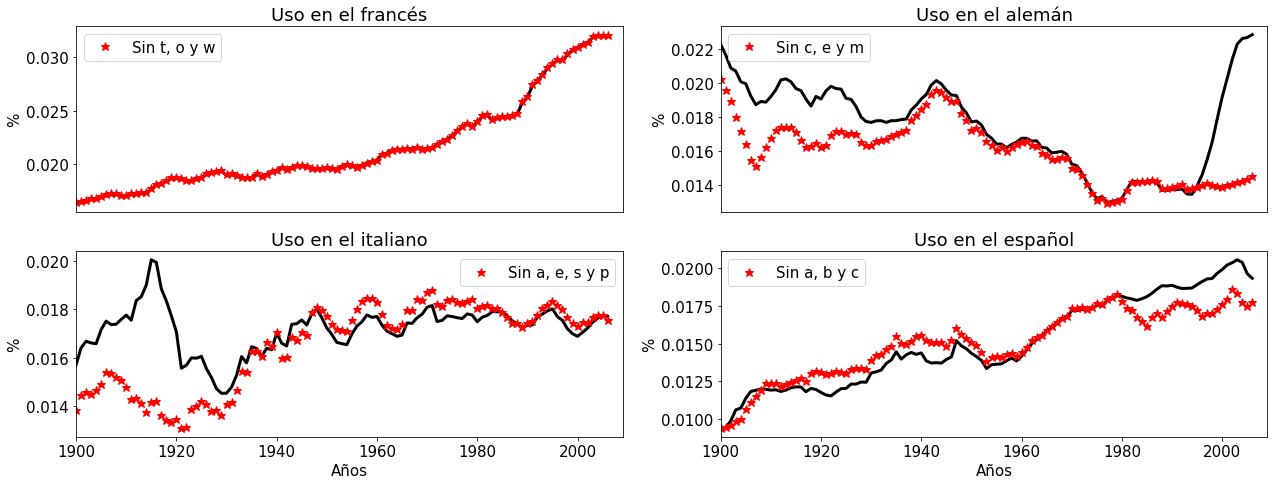
\includegraphics[width=14.5cm, height=6.8cm]{Cap_5/OM_EN.png}
	\label{fig.OM_EN}
	\caption{Omisiones del inglés en los demás.}
\end{figure}


\subsubsection*{Francés}

\begin{figure}[h!]
	\centering
	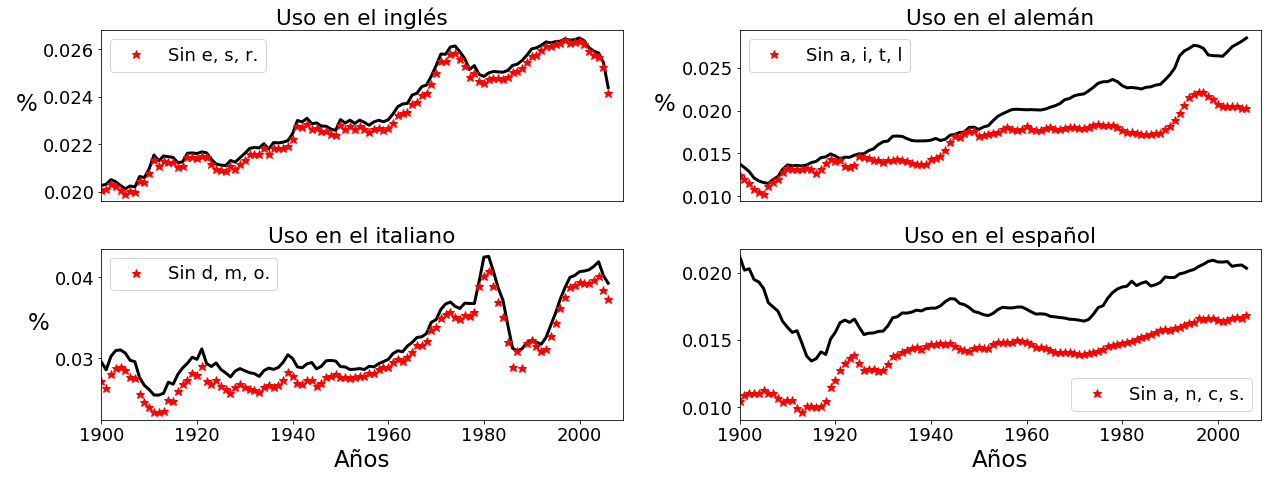
\includegraphics[width=14.5cm, height=6.8cm]{Cap_5/OM_FR.png}
	\label{fig.OM_FR}
	\caption{Omisiones del francés en los demás.}
\end{figure}


\newpage
\subsubsection*{Alemán}

\begin{figure}[h!]
	\centering
	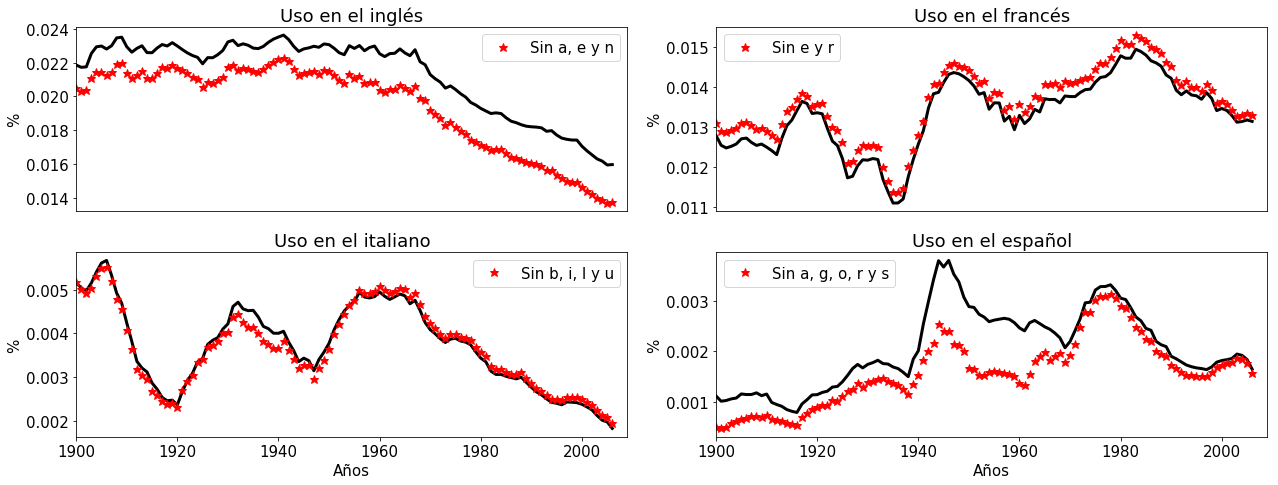
\includegraphics[width=14.5cm, height=6.8cm]{Cap_5/OM_GE.png}
	\label{fig.OM_GE}
	\caption{Omisiones del alemán en los demás.}
\end{figure}


\subsubsection*{Italiano}

\begin{figure}[h!]
	\centering
	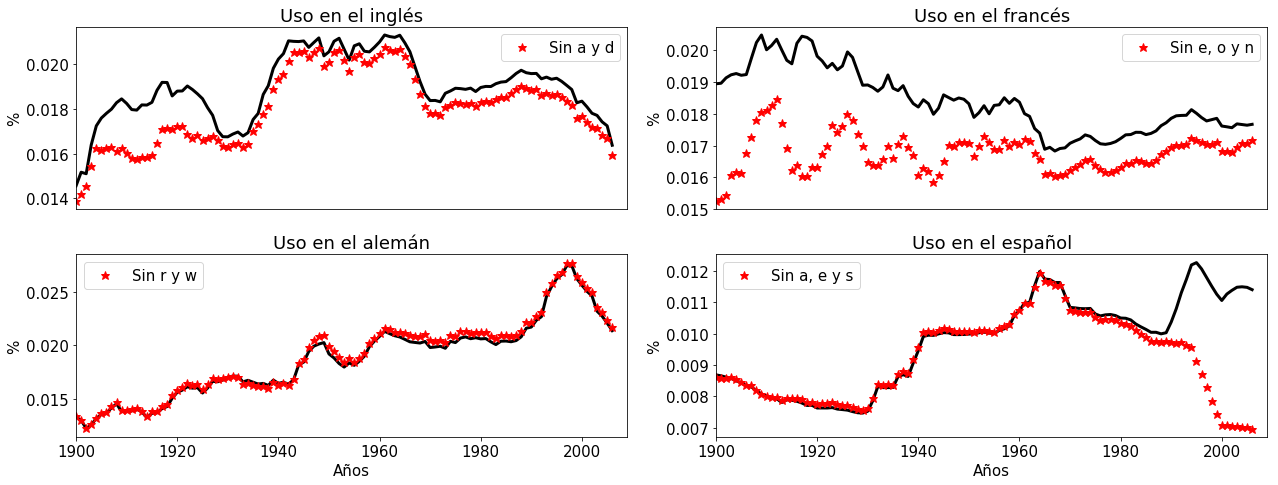
\includegraphics[width=14.5cm, height=6.8cm]{Cap_5/OM_IT.png}
	\label{fig.OM_IT}
	\caption{Omisiones del italiano en los demás.}
\end{figure}

\newpage
\subsubsection*{Español}

\begin{figure}[h!]
	\centering
	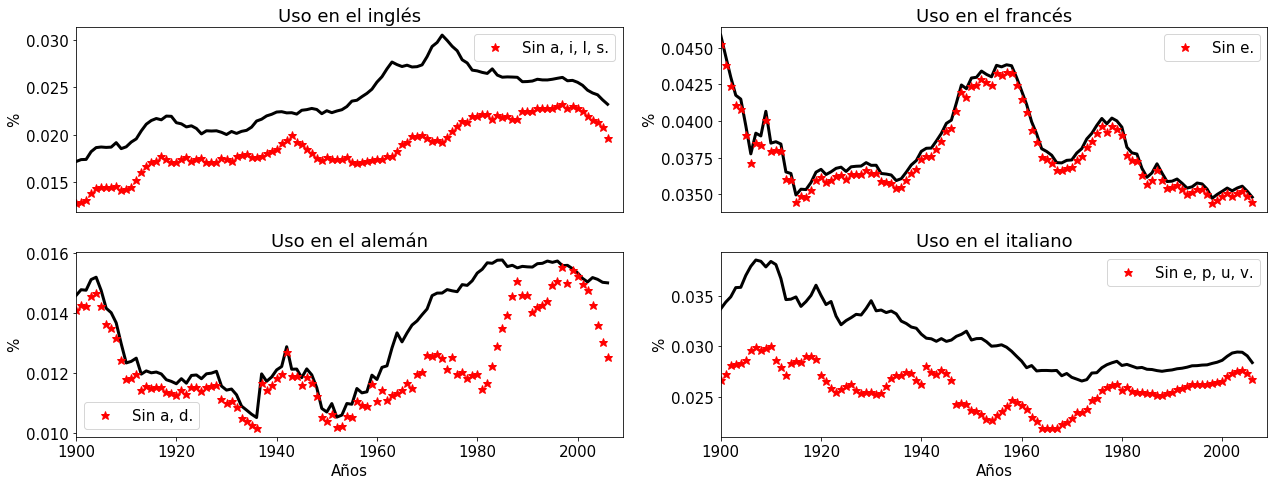
\includegraphics[width=14cm, height=6.8cm]{Cap_5/OM_SP.png}
	\label{fig.OM_SP}
	\caption{Omisiones del español en los demás.}
\end{figure}


\newpage

\begin{table}[h!]
	\centering
	\begin{tabular}{ccc}
		\textbf{}  & \textbf{$\Delta h$}  & \textbf{$R^{2}$}      \\
		\textbf{inglés-francés}    & 0.001           & 0.99       \\
		\textbf{inglés-alemán}     & 0.003           & 0.91       \\
		\textbf{ingles-italiano}   & 0.004           & 0.63       \\
		\textbf{ingles-español}    & 0.002           & 0.93       \\
		\textbf{francés-inglés}    & 0.001           & 0.98       \\    
		\textbf{francés-alemán}    & 0.003           & 0.84       \\ 
		\textbf{francés-italiano}  & 0.002           & 0.81       \\ 
		\textbf{francés-español}   & 0.003           & 0.81       \\ 
		\textbf{alemán-inglés}     & 0.002           & 0.98       \\
		\textbf{alemán-francés}    & 0.002           & 0.88       \\
		\textbf{alemán-italiano}   & 0.001           & 0.99       \\
		\textbf{alemán-español}    & 0.003           & 0.96       \\
		\textbf{italiano-inglés}   & 0.002           & 0.78       \\
		\textbf{italiano-francés}  & 0.003           & 0.79       \\
		\textbf{italiano-alemán}   & 0.001           & 0.97       \\
		\textbf{italiano-español}  & 0.002           & 0.89       \\
		\textbf{español-inglés}    & 0.004           & 0.85       \\
		\textbf{español-francés}   & 0.001           & 0.99       \\
		\textbf{español-alemán}    & 0.003           & 0.67       \\
		\textbf{español-italiano}  & 0.004           & 0.74       
	\end{tabular}
	\caption{Parámetros de las omisiones.}
	\label{tab.Omision}
\end{table}



